% !TEX root = ../main.tex
% --+ 12.21 e- STATISTICS STUDY +-----------------------------------------------
\begin{frame}{$e^-$ Statistics Study}
    \label{12.21::e-_statistics_study}

    After the phase space study, the second criterion to selecting a \textcolor{efd_green}{$7$ cm $v_z$} \ef{region} is maximising statistics.

    \begin{itemize}
        \item
            The length comes from the RG-E target design: \textcolor{efd_green}{3 cm} \ef{long liquid target,} \textcolor{efd_green}{4 cm} \ef{gap, and a solid target of negligible width}.

        \item
            $e^-$ statistics increase the further upstream we go, and thus the selected region is from \ef{$-5$ to $2$} \textcolor{efd_green}{cm}.
    \end{itemize}

    \begin{center}
        \begin{figure}[t]
            \centering{
                \fbox{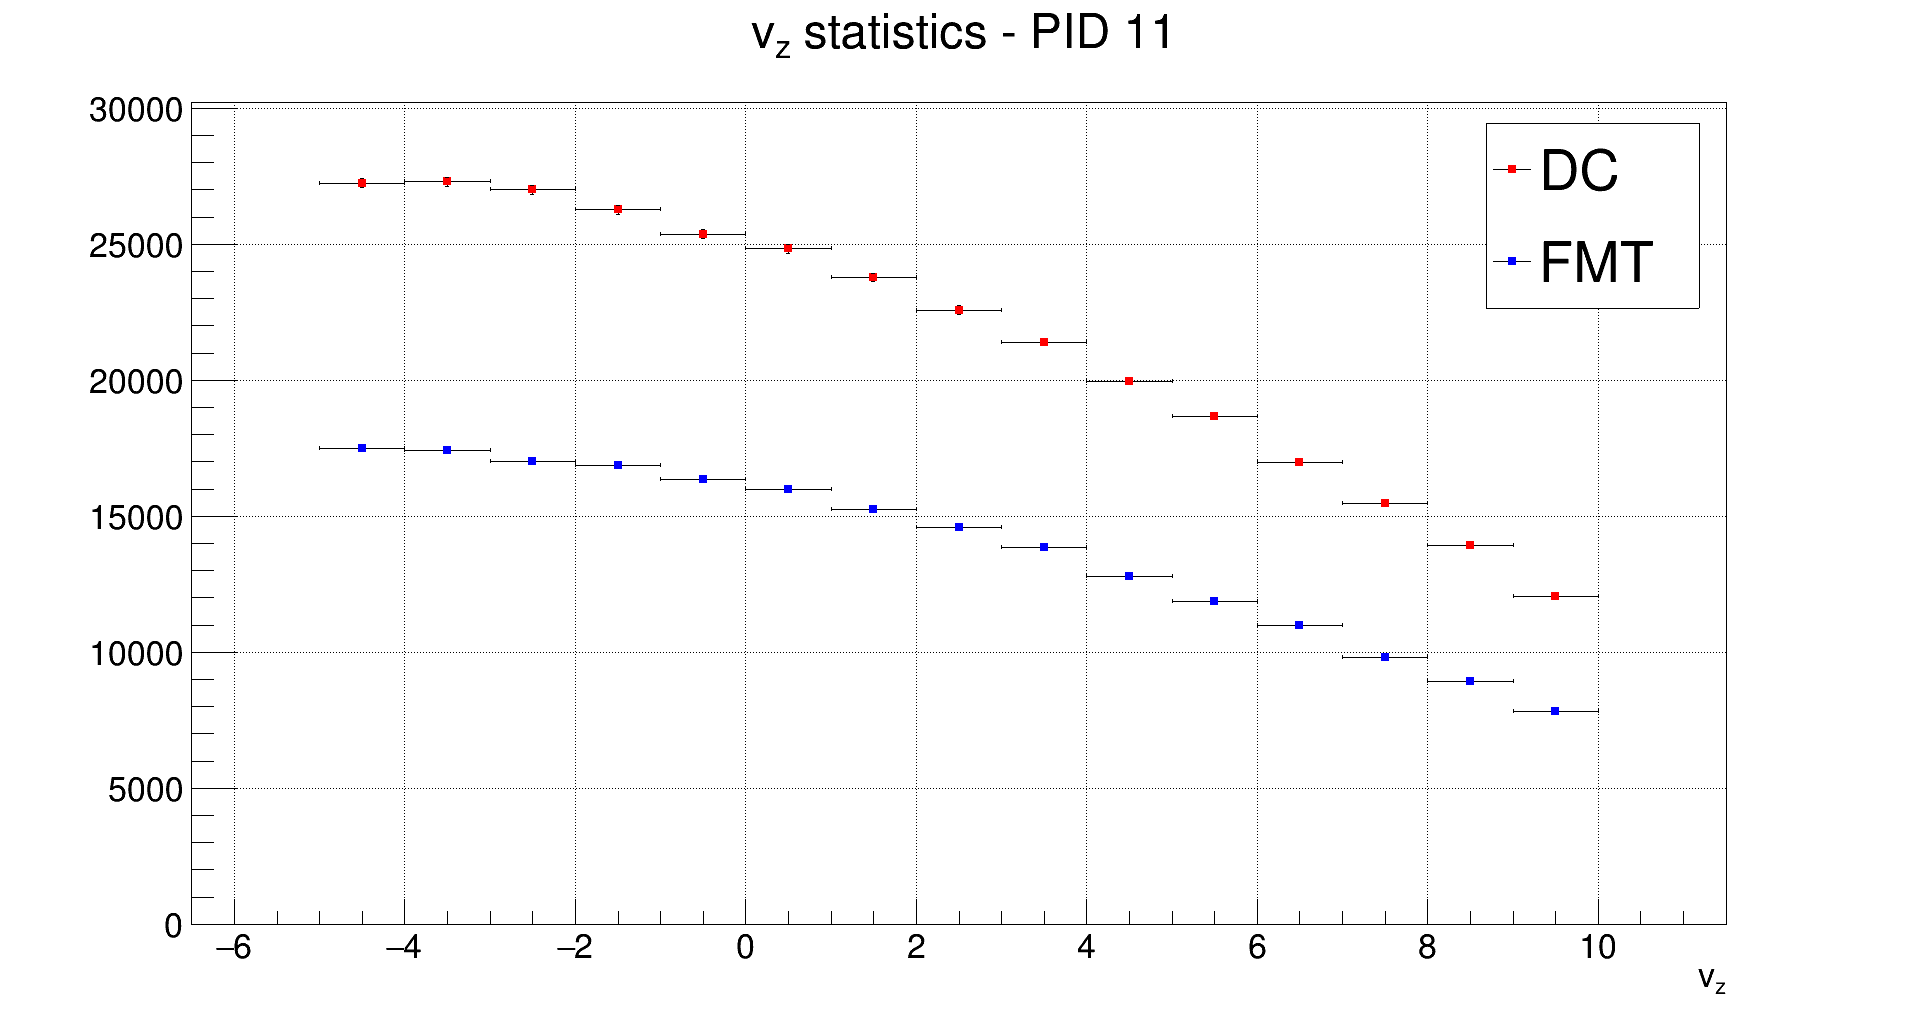
\includegraphics[width=0.6\textwidth]{21statistics_e-.png}}
            }
        \end{figure}
        \scriptsize{\textit{\ef{$v_z$} vs. \ef{$e^-$ statistics}.}}
    \end{center}
\end{frame}

% --+ 12.22 pi STATISTICS STUDY +-----------------------------------------------
\begin{frame}{$e^-\pi^\pm$ Statistics Study}
    \label{12.22::pi_statistics_study}

    The result is only reinforced by \ef{$e^-\pi^+$} and \ef{$e^-\pi^-$ statistics}.

    \vspace{-12pt}

    \begin{columns}[onlytextwidth,T]

    \begin{column}{.49\linewidth}
        \begin{center}
            \begin{figure}[t]
                \centering{
                    \fbox{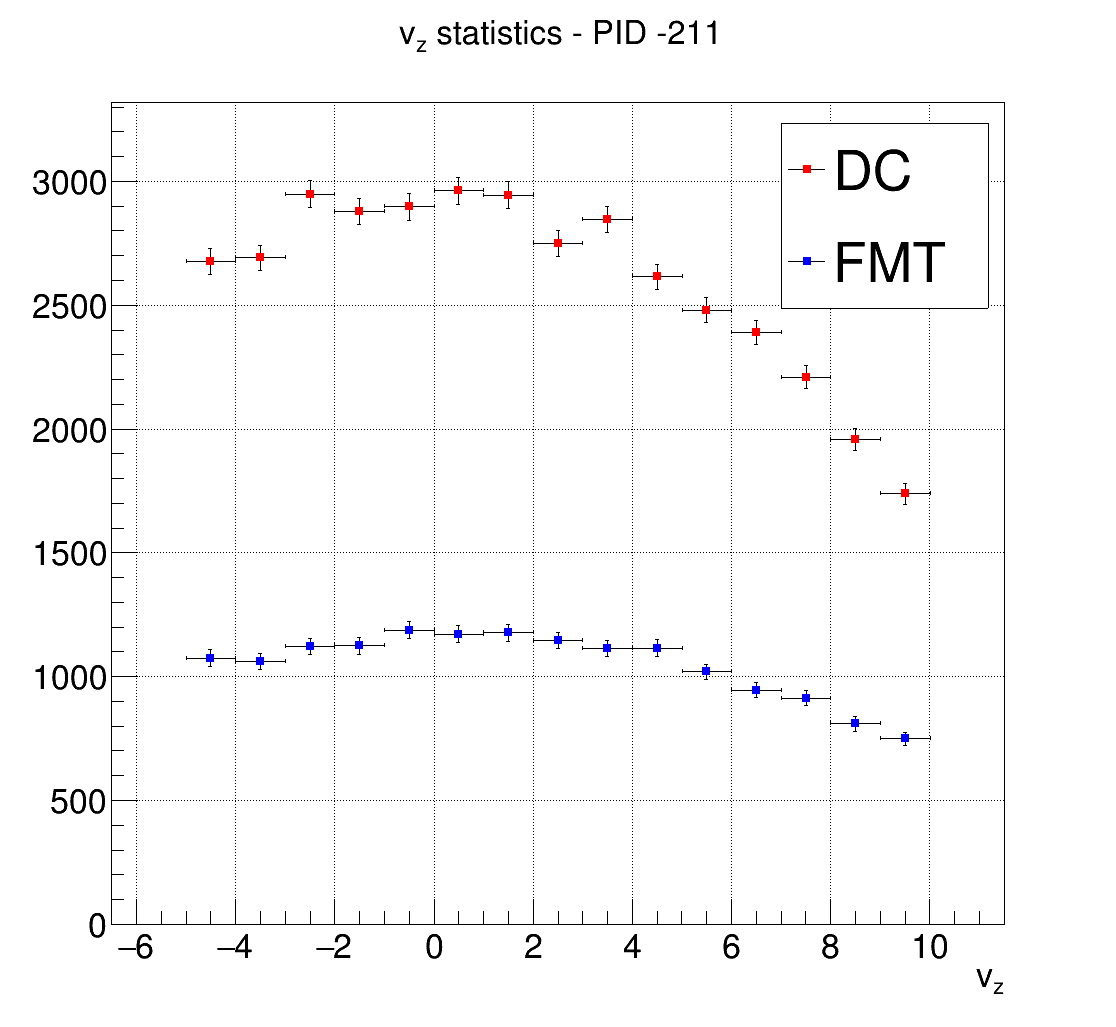
\includegraphics[width=\textwidth]{22statistics_pi-.png}}
                }
            \end{figure}
        \end{center}
    \end{column}

    \begin{column}{.49\linewidth}
        \begin{center}
            \begin{figure}[t]
                \centering{
                    \fbox{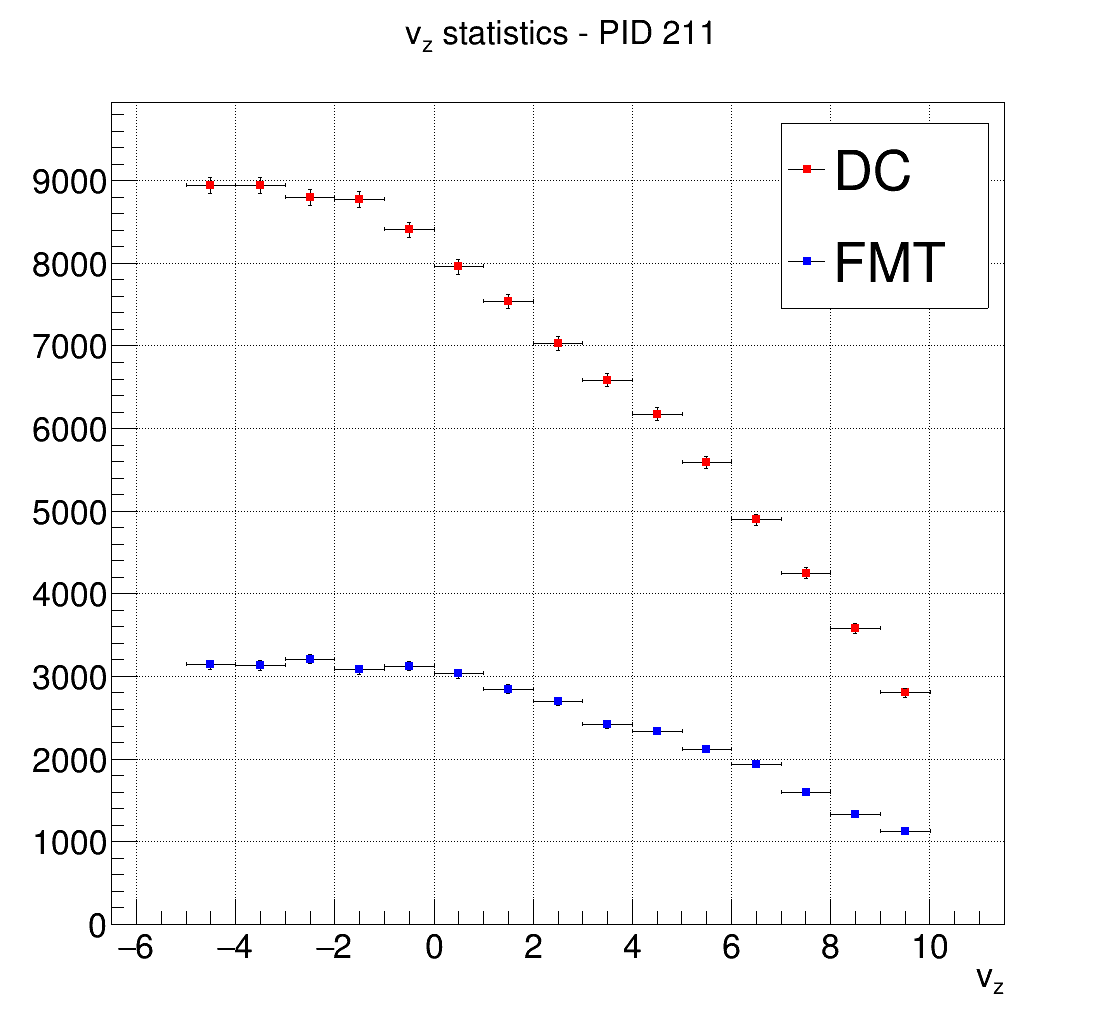
\includegraphics[width=\textwidth]{22statistics_pi+.png}}
                }
            \end{figure}
        \end{center}
    \end{column}

    \end{columns}

    \vspace{-18pt}

    \begin{center}
        \scriptsize{\textit{\ef{$v_z$} vs. \ef{$\pi^+$} and \ef{$\pi^-$} statistics.}}
    \end{center}
\end{frame}
